%% expert_overview.tex
%% Condensed technical reference for expert questionnaire respondents.
%% Compile with: pdflatex expert_overview.tex (standalone, no .bib required)
%%
%% Questionnaire item mapping (shown as [Qn] in section headings):
%%   B1--B4  -> Sections 3, 3.4         (methodology structure, iterative dev.)
%%   B5--B7  -> Sections 3.2, 3.3       (identity model, Root of Trust concept)
%%   B8--B10 -> Sections 3.3, 4.3, 4.4  (RoT execution, protocol phases, hash chain)
%%   B11--B12 -> Sections 3.5, 4.5      (STRIDE, OWASP)
%%   B13--B14 -> Sections 3.1, 5        (tech-agnostic design, comparison table)

\documentclass[12pt,a4paper]{article}

\usepackage[top=2.2cm,bottom=2.2cm,left=2.5cm,right=2.5cm]{geometry}
\usepackage{graphicx}
\usepackage{amsmath,amssymb}
\usepackage{booktabs}
\usepackage{multirow}
\usepackage{array}
\usepackage[table]{xcolor}
\usepackage{makecell}
\usepackage{pifont}
\usepackage{enumitem}
\usepackage{tikz}
\usetikzlibrary{shapes.geometric, arrows.meta, positioning, calc,
                backgrounds, decorations.pathreplacing, fit}
\usepackage[colorlinks=true,linkcolor=blue,urlcolor=blue]{hyperref}
\usepackage{caption}
\usepackage{parskip}
\usepackage{fancyhdr}
\usepackage{mdframed}

%% Check/cross marks
\newcommand{\cmark}{\ding{51}}
\newcommand{\xmark}{\ding{55}}
\definecolor{checkgreen}{RGB}{0,128,0}
\definecolor{crossred}{RGB}{180,0,0}
\definecolor{partialyellow}{RGB}{180,120,0}
\newcommand{\yes}{\textcolor{checkgreen}{\cmark}}
\newcommand{\no}{\textcolor{crossred}{\xmark}}
\newcommand{\pyes}{\textcolor{partialyellow}{\textasciitilde}}

%% Questionnaire item tag (grey label after section title)
\newcommand{\qtag}[1]{\hfill\textcolor{gray!70}{\small\textit{[Questionnaire: #1]}}}

\pagestyle{fancy}
\fancyhf{}
\renewcommand{\headrulewidth}{0.4pt}
\lhead{\small\textit{Expert Validation Reference — IoT Security-by-Design Methodology}}
\rhead{\small\thepage}

% ----------------------------------------------------------------
\begin{document}

\begin{titlepage}
  \centering
  \vspace*{1.5cm}
  {\Large\bfseries Closing the Security Activation Gap:\\[6pt]
   A Security-by-Design Methodology for IoT Ecosystems}\\[0.5cm]
  {\large\bfseries Expert Validation Reference Document}\\[1.5cm]

  {\normalsize
  Raziel Campos-Sánchez$^{1,2}$,\;
  Luis Hernandez-Martinez$^{1}$,\;
  Claudia Feregrino-Uribe$^{2,3}$,\\[4pt]
  Alejandro Penuelas-Angulo$^{4,5}$,\;
  Diego Cruz-Aguilar$^{2,3}$
  }\\[0.8cm]

  {\small
  $^1$ Electronics Department, INAOE, Tonantzintla, Puebla, Mexico\\
  $^2$ Science and Technologies of Security Dept., INAOE\\
  $^3$ Computational Sciences Dept., INAOE\\
  $^4$ CEIT-BRTA, Donostia/San Sebastián, Spain\\
  $^5$ Universidad de Navarra, Tecnum
  }\\[1.5cm]

  \begin{mdframed}[backgroundcolor=blue!4, linecolor=blue!30, linewidth=1pt,
                   innertopmargin=10pt, innerbottommargin=10pt,
                   innerleftmargin=12pt, innerrightmargin=12pt]
  \textbf{Purpose of this document.} This is a condensed technical reference to accompany the expert validation questionnaire. It summarises the methodology, its formal foundations, the case study, and the comparative positioning relative to existing work. The full manuscript is under preparation for submission to \textit{Computers \& Security} (Elsevier, Q1). Sections are cross-referenced with questionnaire items (shown in grey at the right of each heading).
  \end{mdframed}

  \vfill
  {\small Contact: \href{mailto:rcampos@inaoe.mx}{rcampos@inaoe.mx} \hfill \today}
\end{titlepage}

% ----------------------------------------------------------------
\section*{Abstract}

The widespread adoption of IoT ecosystems is constrained by a persistent \emph{security activation gap}: security mechanisms are available in platforms but rarely operational after standard deployment. We present a security-by-design methodology for centralized IoT ecosystems that treats identity as an intrinsic entity property, encompasses seven stages across four phases, and embeds cybersecurity throughout the development lifecycle. A dynamic Root of Trust process establishes verifiable cryptographic identity for each entity before any operational communication begins.

We validate the methodology through a confirmatory case study (Yin, 2014) applying all seven stages to the design and implementation of a DC Smart Microgrid (SMG): three ESP32-based secondary control nodes and a Raspberry Pi~4B primary coordination agent. Results: (CSQ1)~all seven stages produced documented, traceable artifacts; (CSQ2)~a 12-parameter identity model across four entity types was produced without ambiguity; (CSQ3)~the Root of Trust process established mutual authentication with 257.6\,ms total handshake latency and 100\% chain integrity across 400 authenticated messages; (CSQ4)~90\% OWASP IoT Top~10 coverage.

% ----------------------------------------------------------------
\section{Problem and Motivation}
\label{sec:motivation}

A \textbf{security activation gap} exists in IoT deployments: standard deployment activates approximately 3 of 8 available security controls; the remaining 5 require manual post-installation configuration that is rarely performed. This is not a tooling problem---the security mechanisms exist---but a methodological one: cybersecurity is addressed after architectural and technology decisions are made, resulting in bolt-on rather than foundational security.

A second barrier is methodological: most IoT development frameworks treat cybersecurity as an afterthought, lack a formal entity identity model, and provide no empirical validation of their security provisions. A systematic review covering 120+ authentication proposals (2010--2022) confirms that authentication mechanisms are consistently proposed in isolation, without connection to a broader development process or measurable threat coverage metric.

The methodology presented here addresses five dimensions simultaneously that no existing approach covers together: (a)~organizational adoption strategy, (b)~technology-agnostic architectural design with a formal entity-centric identity model, (c)~a dynamic Root of Trust process, (d)~iterative development guided by maturity levels, and (e)~empirical validation through a formal case study with measurable artifacts at every stage.

% ----------------------------------------------------------------
\section{Conceptual Framework}
\label{sec:framework}

Four foundational definitions underpin the methodology, stated independently of any implementation technology.

\begin{description}[leftmargin=0pt, style=nextline]
  \item[\textbf{IoT}] A technological paradigm based on the remote and distributed connectivity of cyber-physical systems equipped with identity, for the purpose of generating and capturing data to convert it into actionable information for intelligent decision-making.

  \item[\textbf{IoT Ecosystem}] A digital environment where elements possess unique identities and interact under a defined structure to provide services that solve identified problems through data collection and intelligent action. The ecosystem comprises seven element types: IoT devices, IoT servers, IoT services, storage systems, users, administrators, and communication infrastructure.

  \item[\textbf{Cybersecurity in an IoT Ecosystem}] Intrinsic properties of the design, development, structure, integration, operation, and physical conditions that determine the vulnerability, robustness, resilience, and response to disturbances or malicious interventions.

  \item[\textbf{Root of Trust Process}] The process by which entities establish, share, and securely store identity parameters in a trusted environment, enabling security mechanisms for IoT ecosystem operations.
\end{description}

The reconceptualization of Root of Trust as a \emph{process} rather than a static hardware component is central to the methodology. It accommodates heterogeneous device capabilities --- from constrained microcontrollers to cloud servers --- and supports both symmetric and asymmetric cryptographic schemes.

% ----------------------------------------------------------------
\section{Proposed Methodology}
\label{sec:methodology}

% ---- 3.1 --------------------------------------------------------
\subsection{Structure: Four Phases and Seven Stages \qtag{B1, B2, B13, B14}}
\label{sec:structure}

The methodology is organized into four phases and seven stages (Figure~\ref{fig:metodologia}). Each stage produces documented outputs that serve as verifiable inputs to the subsequent stage.

\begin{figure}[htbp]
  \centering
  % Figure: Proposed Methodology — 4 phases, 7 stages
% Inline TikZ — vector quality, no external dependencies
%
% Layout: four phase columns side by side with stage boxes inside.
% Horizontal arrows show development flow; dashed arc below shows ITER.

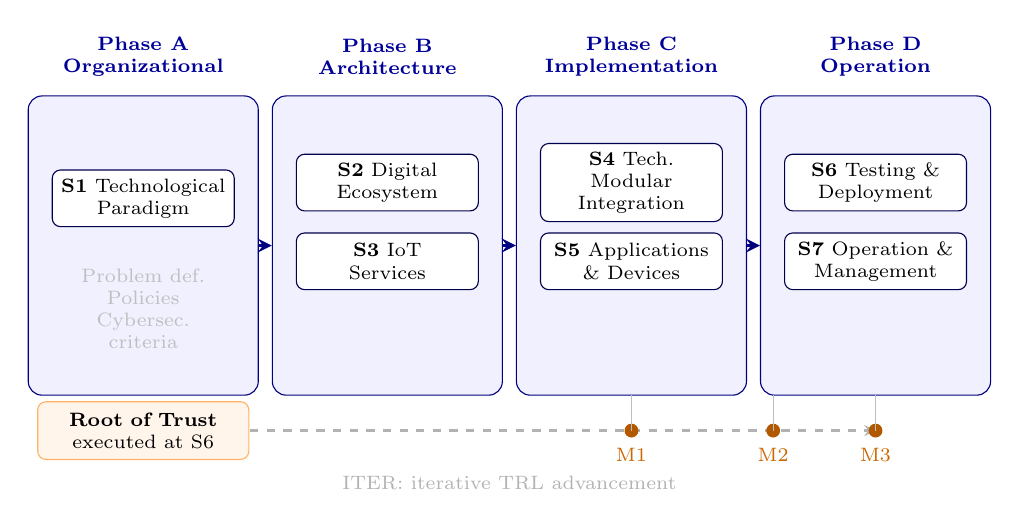
\begin{tikzpicture}[
  font=\small,
  every node/.style={},
  phbox/.style={
    draw=blue!50!black, fill=blue!6, rounded corners=5pt,
    minimum width=2.7cm, text width=2.5cm, minimum height=3.8cm,
    align=center, inner sep=6pt
  },
  phlabel/.style={
    font=\bfseries\scriptsize, text=blue!60!black,
    text width=2.4cm, align=center
  },
  stbox/.style={
    draw=blue!30!black, fill=white, rounded corners=3pt,
    minimum width=2.3cm, text width=2.1cm,
    minimum height=0.72cm, align=center,
    font=\scriptsize, inner sep=3pt
  },
  stno/.style={
    font=\bfseries\scriptsize, text=blue!70!black
  },
  flowarrow/.style={->, very thick, >=stealth, blue!50!black},
  iterarrow/.style={<->, thick, >=stealth, dashed, gray!60},
  maintpt/.style={circle, fill=orange!70!black, minimum size=5pt, inner sep=0}
]

% ── Phase A: Organizational ─────────────────────────────────
\node[phbox] (phA) at (0,0) {};
\node[phlabel] at (0, 2.4) {Phase A\\Organizational};
\node[stbox] at (0, 0.6) {\textbf{S1} Technological\\Paradigm};
\node[font=\scriptsize, text=gray!50, align=center, text width=2.1cm] at (0,-0.8) {Problem def. \\Policies\\Cybersec. criteria};

% ── Phase B: Architecture ───────────────────────────────────
\node[phbox] (phB) at (3.1,0) {};
\node[phlabel] at (3.1, 2.4) {Phase B\\Architecture};
\node[stbox] at (3.1, 0.8) {\textbf{S2} Digital\\Ecosystem};
\node[stbox] at (3.1,-0.2) {\textbf{S3} IoT\\Services};

% ── Phase C: Implementation ─────────────────────────────────
\node[phbox] (phC) at (6.2,0) {};
\node[phlabel] at (6.2, 2.4) {Phase C\\Implementation};
\node[stbox] at (6.2, 0.8) {\textbf{S4} Tech.\ Modular\\Integration};
\node[stbox] at (6.2,-0.2) {\textbf{S5} Applications\\\& Devices};

% ── Phase D: Operation ──────────────────────────────────────
\node[phbox] (phD) at (9.3,0) {};
\node[phlabel] at (9.3, 2.4) {Phase D\\Operation};
\node[stbox] at (9.3, 0.8) {\textbf{S6} Testing \&\\Deployment};
\node[stbox] at (9.3,-0.2) {\textbf{S7} Operation \&\\Management};

% ── Phase flow arrows ────────────────────────────────────────
\draw[flowarrow] (phA.east) -- (phB.west);
\draw[flowarrow] (phB.east) -- (phC.west);
\draw[flowarrow] (phC.east) -- (phD.west);

% ── ITER cycle arc ───────────────────────────────────────────
\draw[iterarrow] (0,-2.35) -- (9.3,-2.35)
    node[pos=0.5, below=0.45cm, font=\scriptsize, text=gray!60] {ITER: iterative TRL advancement};

% ── Maintenance points ───────────────────────────────────────
% M1 fires during implementation (Phase C, x=6.2)
\node[maintpt, label={[font=\scriptsize, text=orange!80!black]below:M1}] at (6.2,-2.35)  {};
% M2 fires during deployment (Phase D, x=8.0)
\node[maintpt, label={[font=\scriptsize, text=orange!80!black]below:M2}] at (8.0,-2.35)  {};
% M3 fires during operation (Phase D, x=9.3)
\node[maintpt, label={[font=\scriptsize, text=orange!80!black]below:M3}] at (9.3,-2.35)  {};

% ── Maintenance point tick lines ─────────────────────────────
\draw[thin, gray!50] (6.2,-1.9) -- (6.2,-2.35);
\draw[thin, gray!50] (8.0,-1.9) -- (8.0,-2.35);
\draw[thin, gray!50] (9.3,-1.9) -- (9.3,-2.35);

% ── RoT highlight note ──────────────────────────────────────
\node[draw=orange!60, fill=orange!8, rounded corners=3pt, font=\scriptsize,
      text width=2.4cm, align=center, inner sep=4pt] at (0,-2.35)
      {\textbf{Root of Trust}\\executed at S6};

\end{tikzpicture}

  \caption{Methodology structure: four phases (A--D) comprising seven stages (S1--S7). ITER cycles advance TRL. Maintenance points M1--M3 trigger targeted stage re-entry.}
  \label{fig:metodologia}
\end{figure}

\textbf{Phase A --- Organizational (Stage~1):} Establishes problem definition, operating policies, development policies (including TRL target), and cybersecurity policies (criticality classification, technological sovereignty, data sovereignty, supply chain risk, regulatory compliance). This phase is unique among IoT methodologies: making cybersecurity constraints explicit at the organizational level before any technology is selected ensures that architectural decisions are security-constrained by design, not patched afterwards.

\textbf{Phase B --- Architecture (Stages~2--3):} Stage~2 defines the ecosystem architecture at the entity level and establishes the formal identity model (Section~\ref{sec:identity}). Stage~3 defines services: secure storage subsystems, access control mechanisms, and identity parameter storage strategies differentiated by device capability (NVS for constrained devices, HSM for servers, MFA for users).

\textbf{Phase C --- Implementation (Stages~4--5):} Stage~4 selects enabling technologies evaluated against maturity (TRL), vulnerability landscape, and supply chain risk. Stage~5 implements all ecosystem elements under secure development guidelines.

\textbf{Phase D --- Operation (Stages~6--7):} Stage~6 covers deployment, Root of Trust execution (Process~6.1.3) for all entities, functional testing, and penetration testing. Stage~7 covers ongoing operation: monitoring, updates, incident response, and threat intelligence.

% ---- 3.2 --------------------------------------------------------
\subsection{Identity Model (Stage~2.2.1) \qtag{B5, B6}}
\label{sec:identity}

Each entity $X$ in ecosystem $E$ possesses an identity defined as:
\begin{equation}
  I^E_X = P^E_{X\;pub} \cup P^E_{X\;priv}
\end{equation}
where $P^E_{X\;pub}$ (public parameters) serve as identifiers and $P^E_{X\;priv}$ (private parameters) enable cryptographic operations. Authentication parameters $P^E_{X\;auth} \subset I^E_X$ and shared secrets $P^E_{X\;SS} \subset P^E_{X\;auth}$ are derived from this foundation. The total parameter count per entity type is:
\begin{equation}
  n^E_X = |P^E_{X\;pub}| + |P^E_{X\;priv}|
\end{equation}

\begin{figure}[htbp]
  \centering
  % Figure: Identity parameter sets
% Nested rectangles: P_SS ⊆ P_auth ⊆ P_priv, with P_pub alongside.
% I^E_X = P_pub ∪ P_priv is the outer container.

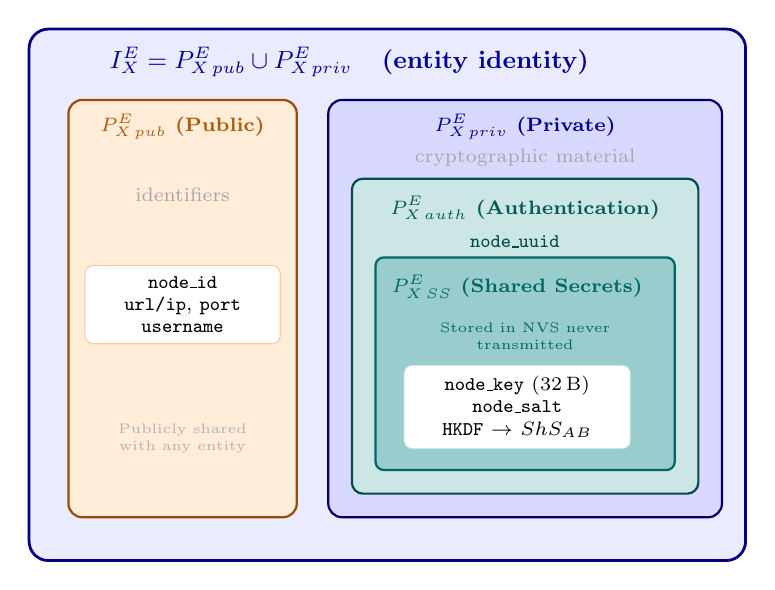
\begin{tikzpicture}[font=\small]

% ── Colour palette ──────────────────────────────────────────
\colorlet{outer}{blue!8}
\colorlet{priv}{blue!15}
\colorlet{auth}{teal!20}
\colorlet{ss}{teal!40}
\colorlet{pub}{orange!15}

% ── Outer identity box: I^E_X ────────────────────────────────
\draw[draw=blue!50!black, fill=outer, rounded corners=7pt, line width=1pt]
    (-0.3, -2.55) rectangle (8.8, 4.2);
\node[font=\bfseries\small, text=blue!60!black, anchor=north west]
    at (0.6, 4.1) {$I^E_X = P^E_{X\,pub} \cup P^E_{X\,priv}$\quad (entity identity)};

% ── P_pub box ───────────────────────────────────────────────
\draw[draw=orange!60!black, fill=pub, rounded corners=5pt, line width=0.8pt]
    (0.2, -2.0) rectangle (3.1, 3.3);
\node[font=\bfseries\scriptsize, text=orange!70!black, anchor=north]
    at (1.65, 3.25) {$P^E_{X\,pub}$ (Public)};
\node[font=\scriptsize, text=gray!70, anchor=north]
    at (1.65, 2.3) {identifiers};
\node[draw=orange!40, fill=white, rounded corners=3pt,
      font=\scriptsize, inner sep=4pt, text width=2.2cm, align=center]
    at (1.65, .7) {\texttt{node\_id}\\\texttt{url/ip}, \texttt{port}\\\texttt{username}};
\node[font=\tiny, text=gray!60, align=center, text width=2.4cm]
    at (1.65, -1.0) {Publicly shared\\with any entity};

% ── P_priv outer box ────────────────────────────────────────
\draw[draw=blue!40!black, fill=priv, rounded corners=5pt, line width=0.8pt]
    (3.5, -2.0) rectangle (8.5, 3.3);
\node[font=\bfseries\scriptsize, text=blue!60!black, anchor=north]
    at (6.0, 3.25) {$P^E_{X\,priv}$ (Private)};
\node[font=\scriptsize, text=gray!70, anchor=north]
    at (6.0, 2.8) {cryptographic material};

% ── P_auth inner box ────────────────────────────────────────
\draw[draw=teal!60!black, fill=auth, rounded corners=4pt, line width=0.8pt]
    (3.8, -1.7) rectangle (8.2, 2.3);
\node[font=\bfseries\scriptsize, text=teal!70!black, anchor=north]
    at (6.0, 2.2) {$P^E_{X\,auth}$ (Authentication)};

% ── P_SS innermost box ──────────────────────────────────────
\draw[draw=teal!80!black, fill=ss, rounded corners=3pt, line width=0.8pt]
    (4.1, -1.4) rectangle (7.9, 1.3);
\node[font=\bfseries\scriptsize, text=teal!80!black, anchor=north]
    at (5.9, 1.2) {$P^E_{X\,SS}$ (Shared Secrets)};
\node[draw=teal!30, fill=white, rounded corners=3pt,
      font=\scriptsize, inner sep=4pt, text width=2.6cm, align=center]
    at (5.9, -0.6) {\texttt{node\_key} (32\,B)\\\texttt{node\_salt}\\\texttt{HKDF} $\rightarrow$ $ShS_{AB}$};

% ── Non-SS auth params label ────────────────────────────────
\node[font=\scriptsize, text=teal!60!black, align=left, text width=1.4cm]
    at (6.0, 1.5) {\texttt{node\_uuid}};

% ── Containment annotations ─────────────────────────────────
\node[font=\tiny, text=teal!80!black, align=center, text width=5.0cm]
    at (6.0, 0.3) {Stored in NVS never\\ transmitted};

\end{tikzpicture}

  \caption{Identity parameter set hierarchy. Shared secrets $P_{SS}$ enable cryptographic operations; $P_{auth}$ proves identity; $P_{priv}$ is never disclosed; $P_{pub}$ serves as identifier.}
  \label{fig:identidad}
\end{figure}

Applying these equations to the SMG produces 12 parameters across 4 entity types with zero overlap (Table~\ref{tab:identity}). The tripartite structure directly determines: what is stored in secure hardware (private/auth parameters), what appears in API calls (public parameters), and what constitutes the authentication proof.

\begin{table}[htbp]
  \centering
  \caption{SMG identity parameter table (Stage~2.2.1 output). \texttt{node\_key}: 32-byte random value generated at provisioning, stored exclusively in ESP32 NVS; never present in \texttt{config.json} or firmware binary.}
  \label{tab:identity}
  \small
  \renewcommand{\arraystretch}{1.2}
  \begin{tabular}{
      >{\raggedright\arraybackslash}p{2.0cm}
      >{\centering\arraybackslash}p{1.3cm}
      >{\raggedright\arraybackslash}p{2.2cm}
      >{\raggedright\arraybackslash}p{2.2cm}
      >{\raggedright\arraybackslash}p{2.2cm}
      >{\centering\arraybackslash}p{0.5cm}
      >{\centering\arraybackslash}p{0.5cm}
      >{\centering\arraybackslash}p{0.8cm}
  }
    \toprule
    \textbf{Entity} & \textbf{Class} & $P_{pub}$ & $P_{priv}$ & $P_{auth}$ & $n$ & $k$ & \textbf{Total} \\
    \midrule
    IoT Node (ESP32) & Device  & \texttt{node\_id} & \texttt{node\_uuid}, \texttt{node\_key} & \texttt{node\_uuid}, \texttt{node\_key} & 1 & 2 & 3 \\
    IoT Server (RPi4) & Server & \texttt{url/ip}, \texttt{port} & \texttt{server\_uuid} & \texttt{server\_uuid} & 2 & 1 & 3 \\
    User             & User   & \texttt{username} & \texttt{user\_uuid}, \texttt{password} & \texttt{user\_uuid}, \texttt{password} & 1 & 2 & 3 \\
    Administrator    & Admin  & \texttt{username} & \texttt{admin\_uuid}, \texttt{password} & \texttt{admin\_uuid}, \texttt{password} & 1 & 2 & 3 \\
    \midrule
    \textbf{Total}   &        & \textbf{5} & \textbf{7} & \textbf{7} & & & \textbf{12} \\
    \bottomrule
  \end{tabular}
\end{table}

% ---- 3.3 --------------------------------------------------------
\subsection{Root of Trust Process \qtag{B7, B8}}
\label{sec:rot}

The Root of Trust process establishes pairwise shared secrets between entities before any network communication. It supports two schemes accommodating heterogeneous device capabilities.

\textbf{Symmetric scheme} (resource-constrained devices): each entity derives a shared secret via HKDF; entities exchange public identifiers and derived secrets; a pairwise key $Key_{ab} = \text{HKDF}(ShS_A \parallel ShS_B)$ is independently computed on both sides. The raw identity key is never transmitted.

\begin{table}[htbp]
  \centering
  \caption{Root of Trust process: symmetric key establishment --- Phase~1 (parameter setup and mutual exchange).}
  \label{tab:rotpsim}
  \small
  \begin{tabular}{
      >{\centering\arraybackslash}p{4.2cm}
      c
      >{\centering\arraybackslash}p{4.8cm}
      c
      >{\centering\arraybackslash}p{4.2cm}
  }
    \toprule
    \textbf{Device} & & \textbf{Message} & & \textbf{Server} \\
    \midrule
    $\{ID_{A},\;MAC_A,\;KEY_A\}$ & & & & $\{ID_B,\;URL/IP_B,\;Port_B,\;KEY_B\}$ \\
    $\text{HKDF}(KEY_A) \rightarrow ShS_A$ & & & & $\text{HKDF}(KEY_B) \rightarrow ShS_B$ \\
    & & $\{ID_A,\;MAC_A,\;ShS_A\} \rightarrow$ & & \\
    & & $\leftarrow \{ID_B,\;URL/IP_B,\;Port_B,\;ShS_B\}$ & & \\
    \bottomrule
  \end{tabular}
\end{table}

\begin{table}[htbp]
  \centering
  \caption{Root of Trust process: symmetric key establishment --- Phase~2 (session key derivation and secure storage; continues Table~\ref{tab:rotpsim}).}
  \label{tab:rotpsim_b}
  \small
  \begin{tabular}{
      >{\centering\arraybackslash}p{3.8cm}
      c
      >{\centering\arraybackslash}p{4.0cm}
      c
      >{\centering\arraybackslash}p{3.8cm}
  }
    \toprule
    \textbf{Device} & & & & \textbf{Server} \\
    \midrule
    $\text{HKDF}(ShS_A \!\parallel\! ShS_B)$ ${\rightarrow\;Key_{ab}}$ & & & & $\text{HKDF}(ShS_A \!\parallel\! ShS_B)$ ${\rightarrow\;Key_{ab}}$ \\
    secure store: $\{Key_{ab},$ $ID_B,\;URL/IP_B,$ $Port_B\}$ & & & & secure store: $\{Key_{ab},\;ID_A,\;MAC_A\}$ \\
    \bottomrule
  \end{tabular}
\end{table}

\textbf{Asymmetric scheme} (capable devices): entities generate public/private key pairs; exchange public keys; store the peer's public key for subsequent ISO/IEC 9798-3 mutual authentication.

\begin{table}[htbp]
  \centering
  \caption{Root of Trust process: asymmetric key establishment.}
  \label{tab:rotpasym}
  \small
  \begin{tabular}{
      >{\centering\arraybackslash}p{3.8cm}
      c
      >{\centering\arraybackslash}p{4.0cm}
      c
      >{\centering\arraybackslash}p{3.8cm}
  }
    \toprule
    \textbf{Device} & & \textbf{Message} & & \textbf{Server} \\
    \midrule
    $\{ID_A,\;MAC_A,$ $PubKey_A,\;PrivKey_A\}$ & & & & $\{ID_B,\;URL/IP_B,$ $Port_B,\;PubKey_B,$ $PrivKey_B\}$ \\
    & & $\{ID_A,\;MAC_A,\;PubKey_A\}$ ${\rightarrow}$ & & \\
    & & ${\leftarrow}$ $\{ID_B,\;URL/IP_B,$ $Port_B,\;PubKey_B\}$ & & \\
    secure store: $\{PubKey_B,$ $ID_B,\;URL/IP_B,\;Port_B\}$ & & & & secure store: $\{PubKey_A,\;ID_A,\;MAC_A\}$ \\
    \bottomrule
  \end{tabular}
\end{table}

The 4-phase execution process is: (1)~prepare identity parameters on isolated workstation, (2)~provision device via trusted physical channel, (3)~exchange public identity information, (4)~derive and securely store pairwise keys. Process~6.1.3 of the methodology mandates execution of this process for \emph{all} entities before the ecosystem goes operational.

% ---- 3.4 --------------------------------------------------------
\subsection{Iterative Development and Maintenance \qtag{B4}}
\label{sec:iter}

The methodology supports TRL-guided iterative cycles (ITER) and three structured maintenance points:
\begin{itemize}[noitemsep]
  \item \textbf{M1} (during implementation): triggers technology re-evaluation when implementation constraints exceed Stage~4 assumptions.
  \item \textbf{M2} (during deployment): triggers code revision when integration testing reveals implementation defects.
  \item \textbf{M3} (during operation): triggers architectural redesign when operational evidence reveals structural limitations.
\end{itemize}

In the SMG case study, three maintenance moments were exercised before deployment: M1 (incorrect HKDF byte slice), M2 (static nonce in session confirmation), M3 (incorrect NVS hex encoding). All were caught through the methodology's stage-transition review requirements.

% ---- 3.5 --------------------------------------------------------
\subsection{STRIDE Threat Coverage \qtag{B11}}
\label{sec:stride}

Table~\ref{tab:stride} maps each STRIDE threat to the methodology stage(s) providing countermeasures, the technology-agnostic mechanism category mandated, and the SMG instantiation. This mapping operates at the methodology level, independently of the specific technologies chosen at Stage~4.

\begin{table*}[htbp]
  \centering
  \caption{STRIDE threat model: mapping to methodology stages. The mechanism category column is technology-agnostic; the SMG instantiation column shows one concrete implementation.}
  \label{tab:stride}
  \small
  \renewcommand{\arraystretch}{1.2}
  \begin{tabular}{
      >{\raggedright\arraybackslash}p{1.7cm}
      >{\raggedright\arraybackslash}p{2.4cm}
      >{\raggedright\arraybackslash}p{2.2cm}
      >{\raggedright\arraybackslash}p{3.1cm}
      >{\raggedright\arraybackslash}p{3.1cm}
      >{\centering\arraybackslash}p{1.5cm}
  }
    \toprule
    \textbf{Threat} & \textbf{Attack Vector} & \textbf{Stage(s)} & \textbf{Mechanism Category} & \textbf{SMG Instantiation} & \textbf{Residual Risk} \\
    \midrule
    \textbf{Spoofing} & Entity impersonation; forged credentials & 2.2.2, 2.2.3, 6.1.3 & Cryptographic mutual authentication using entity-specific shared secrets & PSK + HKDF-SHA256; per-node \texttt{node\_key} in NVS; 3-phase handshake & Low \\
    \midrule
    \textbf{Tampering} & Data modification in transit & 2.2.4, 5.2.1 & Authenticated encryption with integrity binding; random nonces & AES-256-GCM per message; 12-byte random nonce; hash-chain $PRV_{bl}$ & Low \\
    \midrule
    \textbf{Repudiation} & Denial of sent data & 2.2.2, 3.1, 7.1 & Session-bound exchange with archived cryptographic chain & Hash-chain archive on primary server; chain verifiable end-to-end & Low \\
    \midrule
    \textbf{Info.\ Disclosure} & Key extraction; traffic interception & 1.4.2--1.4.3, 2.2.1, 5.2.1 & Data sovereignty policy; private params isolated; app-layer encryption & \texttt{node\_key} in NVS only; all data AES-256-GCM encrypted in transit & Low \\
    \midrule
    \textbf{Denial of Service} & Auth flooding; node isolation & 7.1, 7.2.1, 2.1.8 & Anomaly-based trust scoring; degraded-mode operation; entity isolation & Trust score decay; UNTRUSTED nodes isolated (TCP dropped) & Medium \\
    \midrule
    \textbf{Elev.\ of Privilege} & Node masquerading as admin & 2.1.8, 3.2.1, 2.2.2 & Entity type hierarchy; API-enforced access control & Node tokens permit POST sensor data only; admin endpoints reject node tokens & Low \\
    \bottomrule
  \end{tabular}
\end{table*}

% ----------------------------------------------------------------
\section{Case Study: DC Smart Microgrid}
\label{sec:casestudy}

The case study follows a \textbf{confirmatory design} (Yin, 2014): the methodology is the theoretical proposition; the SMG implementation is the empirical test.

\textbf{Hardware:} Three ESP32 NodeMCU secondary control nodes (dual-core 240\,MHz, 520\,KB SRAM, built-in WiFi) + Raspberry Pi~4B primary coordination agent. Each node includes: local 12\,V AGM battery, $\times$3 DC-DC SSRs for energy flow control, ACS712 current sensors, and a resistive voltage divider for bus monitoring. The SMG is classified as \textbf{critical infrastructure} (Stage~1, Process~1.4.1), requiring the highest cybersecurity tier.

\textbf{Software:} ESP32 firmware: MicroPython 1.22.1 with 4 modules (sensor, EMS, security, communications) + metrics collection. RPi4B server: REST API, time-series database, monitoring dashboard, and a 27-rule security-aware fuzzy Energy Management System. Development target: TRL~3 (proof of concept with physical elements).

% ---- 4.1 --------------------------------------------------------
\subsection{Stage-by-Stage Traceability \qtag{B1, B3}}
\label{sec:traceability}

Tables~\ref{tab:traceability_a} and~\ref{tab:traceability_b} document the application of each methodology stage to the SMG. All 7 stages produced verifiable artifacts (14 distinct outputs) with no design decisions required outside what the methodology's processes prescribe.

\begin{table*}[htbp]
  \centering
  \caption{Stage-by-stage traceability (Part~1, Stages~1--3): methodology process $\rightarrow$ SMG decision $\rightarrow$ artifact. Evidence for CSQ1.}
  \label{tab:traceability_a}
  \small
  \renewcommand{\arraystretch}{1.15}
  \begin{tabular}{
      >{\centering\arraybackslash}p{1.4cm}
      >{\raggedright\arraybackslash}p{3.0cm}
      >{\raggedright\arraybackslash}p{4.7cm}
      >{\raggedright\arraybackslash}p{4.0cm}
  }
    \toprule
    \textbf{Stage} & \textbf{Methodology Process} & \textbf{Decision Made in SMG} & \textbf{Artifact} \\
    \midrule
    \multirow{4}{=}{\textbf{1} Paradigm}
        & 1.1 Establish problem & Manage distributed renewable energy nodes securely in a 12\,V DC microgrid & Problem specification \\
        & 1.1.2 Entities & 5 entity types: IoT nodes, server, users, admins, DC bus & Entity list \\
        & 1.4.1 Criticality & Classified as critical infrastructure & High-security cybersecurity policy \\
        & 1.4.2 Sovereignty & Self-hosted; no third-party cloud & Architecture constraint record \\
    \midrule
    \multirow{5}{=}{\textbf{2} Ecosystem}
        & 2.1.4 Topology & Centralized: all nodes report to primary agent & Architecture diagram \\
        & 2.1.7 Processing & Fog: local EMS on ESP32; global on RPi4 & Processing topology record \\
        & 2.2.1 Identity & 4 entity types $\times$ 3 parameters = 12 identity parameters & Identity parameter table \\
        & 2.2.2 Auth.\ mech. & PSK mutual auth via HKDF-SHA256; AES-256-GCM session & Authentication diagram \\
        & 2.2.3 RoT & 4-phase RoT for node--server pairs & RoT execution log \\
    \midrule
    \multirow{2}{=}{\textbf{3} Services}
        & 3.1 Services & 4 services: data, EMS, auth API, monitoring & Service specification \\
        & 3.2.1 Access ctrl & Token-based; nodes: POST only; users: GET; admins: full & Access control matrix \\
    \bottomrule
  \end{tabular}
\end{table*}

\begin{table*}[htbp]
  \centering
  \caption{Stage-by-stage traceability (Part~2, Stages~4--7): continued from Table~\ref{tab:traceability_a}.}
  \label{tab:traceability_b}
  \small
  \renewcommand{\arraystretch}{1.15}
  \begin{tabular}{
      >{\centering\arraybackslash}p{1.4cm}
      >{\raggedright\arraybackslash}p{3.0cm}
      >{\raggedright\arraybackslash}p{4.7cm}
      >{\raggedright\arraybackslash}p{4.0cm}
  }
    \toprule
    \textbf{Stage} & \textbf{Methodology Process} & \textbf{Decision Made in SMG} & \textbf{Artifact} \\
    \midrule
    \multirow{4}{=}{\textbf{4} Tech.\ Int.}
        & 4.1.1 TRL & TRL~3 target for ITER~1 & TRL milestone record \\
        & 4.1.2 Platform & ESP32 + MicroPython: WiFi built-in, SHA-256 HW, NVS & Technology selection rationale \\
        & 4.1.3 Comms & WiFi 802.11\,b/g/n + TCP; application-layer PSK & Protocol selection record \\
        & 4.2 CVE assessment & ESP32-IDF5 CVEs assessed; MicroPython 1.22.1 pinned & Risk register \\
    \midrule
    \multirow{3}{=}{\textbf{5} Apps \& Dev.}
        & 5.1.1 Server & REST API + time-series DB + dashboard on RPi4 & Server deployment \\
        & 5.1.2 Devices & ESP32 MicroPython firmware: 4 modules & Firmware artifact \\
        & 5.2.1 Secure dev. & NVS for all secrets; \texttt{os.urandom(12)} nonces; no credentials in source & Code review record \\
    \midrule
    \multirow{3}{=}{\textbf{6} Testing}
        & 6.1.3 RoT exec. & RoT executed for all 3 nodes at deployment & Deployment log (3 entries) \\
        & 6.2.1 Functional & 8 functional tests: all pass on all 3 nodes & Test report (8/8 pass) \\
        & 6.2.2 Pen.\ test & NVS parameter tampering $\Rightarrow$ auth failure confirmed & Security verification log \\
    \midrule
    \multirow{2}{=}{\textbf{7} Operation}
        & 7.1.1 Monitoring & Real-time V, I, P, PWM, auth status, session history & Dashboard artifact \\
        & 7.2.2 Updates & OTA update policy with authentication requirement (ITER~2 target) & Update policy \\
    \bottomrule
  \end{tabular}
\end{table*}

% ---- 4.2 --------------------------------------------------------
\subsection{Authentication Protocol Phases P1--P6 \qtag{B9, B10}}
\label{sec:phases}

The SMG implements the Root of Trust through six protocol phases chosen at Stage~4. These constitute an \emph{implementation-specific} technology choice, not a methodology contribution; any protocol providing equivalent mechanism categories would satisfy the same properties. Table~\ref{tab:phases} describes each phase.

\begin{table*}[htbp]
  \centering
  \caption{SMG authentication protocol phases (P1--P6). STRIDE: S~=~Spoofing, T~=~Tampering, R~=~Repudiation, ID~=~Info.\ Disclosure, DoS~=~Denial of Service, EoP~=~Elev.\ of Privilege.}
  \label{tab:phases}
  \small
  \renewcommand{\arraystretch}{1.2}
  \begin{tabular}{
      >{\centering\arraybackslash}p{0.5cm}
      >{\raggedright\arraybackslash}p{1.9cm}
      >{\raggedright\arraybackslash}p{2.0cm}
      >{\raggedright\arraybackslash}p{5.4cm}
      >{\centering\arraybackslash}p{1.9cm}
      >{\centering\arraybackslash}p{1.5cm}
  }
    \toprule
    \textbf{Ph.} & \textbf{Name} & \textbf{Security Role} & \textbf{Mechanism} & \textbf{STRIDE} & \textbf{OWASP} \\
    \midrule
    P1 & Provisioning & Identity before network exposure & \texttt{node\_key} (\texttt{os.urandom(32)}), \texttt{node\_uuid} (UUID-4), WiFi credentials written to ESP32 NVS via USB on isolated workstation; absent from \texttt{config.json} and firmware & S, ID & I1, I9 \\
    \midrule
    P2 & Root of Trust & Pairwise key derivation without key transmission & HKDF-SHA256 (RFC~5869): $ShS_A \leftarrow \text{HKDF}(salt, key)$; both sides independently compute $ShS_{AB} \leftarrow \text{SHA-256}(ShS_A \| ShS_B)$; raw key never transmitted & S & I1, I3 \\
    \midrule
    P3 & Session Estab. & Mutual auth + session-key agreement & 5-message PSK handshake; $SES_{key} \leftarrow \text{SHA-256}(RDN2 \| ShS_{AB})$; AES-256-GCM confirmation; both parties verify shared-secret knowledge without transmitting it & S, T, ID & I2, I3 \\
    \midrule
    P4 & Data Exchange & Per-message authenticated encryption + integrity chain & $c_i \leftarrow \text{AES-256-GCM}(SES_{key}, \text{nonce}_i, m_i)$ with $\text{nonce}_i = \texttt{os.urandom(12)}$; hash chain $PRV_{bl} \leftarrow \text{SHA-256}(PRV_{bl} \| c_i)$; message counter enforces ordering & T, R, ID & I2, I7 \\
    \midrule
    P5 & Logout & Session teardown + verifiable archival & Session state cleared from node memory; chain record $(M_{num}, PRV_{bl}, \text{timestamps})$ archived on server under \texttt{node\_id} & R & I8 \\
    \midrule
    P6 & Chain Audit & Retrospective integrity verification & Server recomputes $PRV_{bl}$ chain from session start; any modified, inserted, or dropped message breaks the chain; independent of node participation & T, R & I7, I8 \\
    \bottomrule
  \end{tabular}
\end{table*}

% ---- 4.3 --------------------------------------------------------
\subsection{Performance Measurements \qtag{B8, B9, B10}}
\label{sec:measurements}

Table~\ref{tab:csq3} reports measurements from a 400-send bench trial on SMG\_NODE\_01 (firmware identical across all three nodes). One mid-trial WiFi reconnect at message 381 inflates the P4 and send-latency standard deviations. $V_{bus}$, tracking error, and node power require physical bus connection (deferred to ITER~2).

\begin{table}[htbp]
  \centering
  \caption{Security and performance measurements (400-send bench trial, 2026-06-22, SMG\_NODE\_01).}
  \label{tab:csq3}
  \small
  \renewcommand{\arraystretch}{1.2}
  \begin{tabular}{
      >{\raggedright\arraybackslash}p{5cm}
      >{\centering\arraybackslash}p{3cm}
      >{\raggedright\arraybackslash}p{5.5cm}
  }
    \toprule
    \textbf{Metric} & \textbf{Value} & \textbf{Notes} \\
    \midrule
    Actual sampling rate (Hz)               & 2.49                  & Target: 3\,Hz \\
    Sensor read avg $\pm$ std ($\mu$s)      & $174\,396 \pm 3\,112$ & 16-sample median oversampling \\
    EMS inference avg $\pm$ std ($\mu$s)    & $1\,046 \pm 357$      & 9-rule Mamdani centroid \\
    P2 RoT latency (ms)                     & 167.1                 & HKDF-SHA256 + 1 WiFi RTT \\
    P3 session latency (ms)                 & 90.3                  & PSK handshake + 2 WiFi RTTs \\
    Handshake total P2+P3 (ms)              & 257.6                 & Dominated by WiFi RTT, not crypto \\
    P4 per-message avg $\pm$ std (ms)       & $52.7 \pm 177.4$      & Std inflated by 1 reconnect outlier \\
    Data payload avg (bytes)                & 156.3                 & JSON sensor data + P4 ciphertext \\
    Chain length                            & 400                   & Verified P4 messages \\
    Send success rate                       & 99.8\%                & 398/400 successful \\
    Chain integrity                         & 100\%                 & P6 hash-chain audit \\
    Heap at boot (B)                        & $88\,832$             & Before module imports \\
    Heap at session (B)                     & $79\,584$             & Post-handshake \\
    Free heap at shutdown (B)               & $73\,840$             & \texttt{gc.mem\_free()} \\
    Heap drift per 100 loops (B)            & $-123.2$              & $<$0.5\% of available heap \\
    Security errors                         & 0                     & Auth + chain failures \\
    $V_{bus}$ mean $\pm$ std (V)            & ---                   & Requires physical SMG bus (ITER~2) \\
    $V_{bus}$ tracking error (V)            & ---                   & Requires physical SMG bus (ITER~2) \\
    Node power (W)                          & ---                   & Requires physical SMG bus (ITER~2) \\
    \bottomrule
  \end{tabular}
\end{table}

% ---- 4.4 --------------------------------------------------------
\subsection{OWASP IoT Top~10 Coverage \qtag{B12}}
\label{sec:owasp}

Table~\ref{tab:owasp} maps each OWASP IoT Top~10 item to the methodology stage(s) and protocol phase(s) providing the countermeasure. 9 of 10 items are fully addressed; the single partial item (I10: physical hardening) is inherently outside the scope of a software development methodology.

\begin{table*}[htbp]
  \centering
  \caption{OWASP IoT Top~10 coverage. Stage = methodology stage. Phase(s) = SMG protocol phase providing implementation evidence. --- = addressed by policy, not protocol.}
  \label{tab:owasp}
  \small
  \renewcommand{\arraystretch}{1.2}
  \begin{tabular}{
      >{\centering\arraybackslash}p{0.4cm}
      >{\raggedright\arraybackslash}p{2.2cm}
      >{\centering\arraybackslash}p{1.4cm}
      >{\centering\arraybackslash}p{1.4cm}
      >{\raggedright\arraybackslash}p{5.8cm}
      >{\centering\arraybackslash}p{1.2cm}
  }
    \toprule
    \textbf{\#} & \textbf{OWASP IoT Risk} & \textbf{Stage(s)} & \textbf{Phase(s)} & \textbf{Evidence in SMG} & \textbf{Cvg.} \\
    \midrule
    I1 & Weak/hardcoded passwords & 2.2.1 & P1, P2 & \texttt{node\_key} = \texttt{os.urandom(32)} at provisioning; stored in NVS only; P2 derives session key without transmitting it & Full \\
    I2 & Insecure network services & 2.2.4 & P3, P4 & P3 establishes AES-256-GCM session before data accepted; P4 encrypts every message with per-message nonce; no plaintext channel & Full \\
    I3 & Insecure ecosystem interfaces & 3.2.1 & P2, P3 & P2+P3 mutual authentication; entity-type access control on all API endpoints; trust score $<0.30$ disconnects anomalous nodes & Full \\
    I4 & Lack of secure update & 7.2.2 & --- & OTA update policy (Stage~7.2.2): admin auth + firmware signature required; implementation scoped to ITER~2 & Full \\
    I5 & Insecure/outdated components & 4.2 & --- & ESP32-IDF5 CVE assessment; MicroPython~1.22.1 pinned; no deprecated crypto (all: HKDF-SHA256, AES-256-GCM, SHA-256 HW) & Full \\
    I6 & Insufficient privacy & 1.4.3 + 2.2.4 & P4 & Self-hosted RPi4; no PII; P4 encrypts all telemetry with authenticated encryption & Full \\
    I7 & Insecure data transfer/storage & 3.1.1 + 2.2.4 & P4, P6 & P4 AES-256-GCM per message; P6 chain audit; \texttt{node\_key} in NVS; no secrets in \texttt{config.json} & Full \\
    I8 & Lack of device management & 7.1 & P5, P6 & Stage~7.1 monitors chain length, heap, send rate; P5 archives session lifecycle; P6 provides complete verifiable audit trail & Full \\
    I9 & Insecure default settings & 2.2.3 + 6.1.3 & P1 & \texttt{machine.reset()} fires if no NVS identity; unique parameters per node at provisioning; no factory defaults & Full \\
    I10 & Lack of physical hardening & --- & --- & Outside software methodology scope; addressed at org.\ level (Stage~1.4.1); JTAG disable and secure boot for TRL~5+ & Partial \\
    \midrule
    & \textbf{Coverage score} & & & & \textbf{9/10} \\
    \bottomrule
  \end{tabular}
\end{table*}

% ----------------------------------------------------------------
\section{Comparison with Related Work \qtag{B14}}
\label{sec:comparison}

Table~\ref{tab:metodologias} compares the proposed methodology against representative existing approaches across nine criteria. A 2023 comparative review confirms that cybersecurity integration remains the most underdeveloped dimension across IoT development methodologies. The proposed methodology is the only approach achieving full coverage across all nine criteria, including the ninth criterion (security validation through a formal case study), which \emph{no} existing methodology addresses.

\begin{table*}[htbp]
  \centering
  \caption{Comparison of IoT development methodologies (9 criteria). \yes~full, \pyes~partial, \no~absent. Sec.Val.~= security provisions validated through formal case study or experiment. Org.~= organizational aspects. Maturity~= TRL or equivalent framework.}
  \label{tab:metodologias}
  \small
  \resizebox{\textwidth}{!}{%
  \begin{tabular}{|l|c|c|c|c|c|c|c|c|c|}
    \hline
    \textbf{Methodology} & \makecell{Tech.\\Dev.} & \makecell{Cyber\\Sec.} & \makecell{Agnostic} & \makecell{Org.} & \makecell{Scal-\\ability} & \makecell{Maturity} & \makecell{Inter-\\op.} & \makecell{Concept.\\Frame.} & \makecell{Sec.\\Val.} \\
    \hline
    Manate et al.\ (2014)          & \pyes & \pyes & \no   & \no   & \yes  & \no   & \yes  & \no   & \no \\
    \hline
    Ayala et al.\ (2015)           & \yes  & \no   & \yes  & \no   & \pyes & \no   & \yes  & \pyes & \no \\
    \hline
    Spanoudakis et al.\ (2015)     & \yes  & \no   & \no   & \pyes & \yes  & \no   & \yes  & \no   & \no \\
    \hline
    Patel et al.\ (2015)           & \yes  & \no   & \no   & \no   & \yes  & \no   & \yes  & \yes  & \no \\
    \hline
    Costa et al.\ (2016)           & \yes  & \no   & \no   & \no   & \yes  & \no   & \yes  & \no   & \no \\
    \hline
    Fortino et al.\ (2017)         & \yes  & \no   & \no   & \no   & \yes  & \yes  & \yes  & \no   & \no \\
    \hline
    Josyula et al.\ (2017)         & \no   & \yes  & \yes  & \no   & \yes  & \no   & \yes  & \no   & \no \\
    \hline
    Savaglio et al.\ (2018)        & \pyes & \pyes & \yes  & \no   & \yes  & \no   & \yes  & \pyes & \no \\
    \hline
    Casadei et al.\ (2019)         & \yes  & \no   & \pyes & \no   & \yes  & \no   & \yes  & \pyes & \no \\
    \hline
    Guerrero-Ulloa et al.\ (2023)  & \yes  & \no   & \yes  & \pyes & \pyes & \no   & \pyes & \no   & \no \\
    \hline
    Muñoz et al.\ (2025)           & \yes  & \pyes & \no   & \no   & \pyes & \no   & \pyes & \pyes & \no \\
    \hline
    \rowcolor{blue!6}
    \textbf{This work (2026)}      & \pyes & \yes  & \yes  & \yes  & \yes  & \yes  & \yes  & \yes  & \yes \\
    \hline
  \end{tabular}}
\end{table*}

Key differentiators relative to the closest existing approaches:
\begin{itemize}[noitemsep]
  \item \textbf{vs.\ Josyula (2017):} Josyula defines processes at a general level with no identity model and no technology selection guidance. This work provides a formal 12-parameter identity model and a stage-by-stage technology evaluation process.
  \item \textbf{vs.\ Savaglio (2018):} Savaglio includes security aspects (key management, authentication) in a reference architecture but does not define selection criteria or specify when controls are applied relative to development stages.
  \item \textbf{vs.\ Muñoz (2025):} Muñoz proposes a 5-layer architecture with security as a cross-cutting concern but does not explain mechanism selection and its PKI-based scheme excludes resource-constrained devices.
  \item \textbf{All existing approaches:} No existing methodology provides empirical validation of its security provisions through a formal case study with measurable artifacts. This is the first methodology to achieve Sec.Val. = \yes.
\end{itemize}

\vfill
\noindent\rule{\textwidth}{0.4pt}\\[4pt]
{\small \textbf{Correspondence:} Raziel Campos-Sánchez --- \href{mailto:rcampos@inaoe.mx}{rcampos@inaoe.mx} --- INAOE, Tonantzintla, Puebla, Mexico.\\
\textbf{Manuscript target:} \textit{Computers \& Security}, Elsevier (Q1, IF\,$\approx$\,5.6). Submission pending expert questionnaire responses.}

\end{document}
